% Options for packages loaded elsewhere
\PassOptionsToPackage{unicode}{hyperref}
\PassOptionsToPackage{hyphens}{url}
%
\documentclass[
  ,man]{apa6}
\usepackage{amsmath,amssymb}
\usepackage{lmodern}
\usepackage{iftex}
\ifPDFTeX
  \usepackage[T1]{fontenc}
  \usepackage[utf8]{inputenc}
  \usepackage{textcomp} % provide euro and other symbols
\else % if luatex or xetex
  \usepackage{unicode-math}
  \defaultfontfeatures{Scale=MatchLowercase}
  \defaultfontfeatures[\rmfamily]{Ligatures=TeX,Scale=1}
\fi
% Use upquote if available, for straight quotes in verbatim environments
\IfFileExists{upquote.sty}{\usepackage{upquote}}{}
\IfFileExists{microtype.sty}{% use microtype if available
  \usepackage[]{microtype}
  \UseMicrotypeSet[protrusion]{basicmath} % disable protrusion for tt fonts
}{}
\makeatletter
\@ifundefined{KOMAClassName}{% if non-KOMA class
  \IfFileExists{parskip.sty}{%
    \usepackage{parskip}
  }{% else
    \setlength{\parindent}{0pt}
    \setlength{\parskip}{6pt plus 2pt minus 1pt}}
}{% if KOMA class
  \KOMAoptions{parskip=half}}
\makeatother
\usepackage{xcolor}
\usepackage{graphicx}
\makeatletter
\def\maxwidth{\ifdim\Gin@nat@width>\linewidth\linewidth\else\Gin@nat@width\fi}
\def\maxheight{\ifdim\Gin@nat@height>\textheight\textheight\else\Gin@nat@height\fi}
\makeatother
% Scale images if necessary, so that they will not overflow the page
% margins by default, and it is still possible to overwrite the defaults
% using explicit options in \includegraphics[width, height, ...]{}
\setkeys{Gin}{width=\maxwidth,height=\maxheight,keepaspectratio}
% Set default figure placement to htbp
\makeatletter
\def\fps@figure{htbp}
\makeatother
\setlength{\emergencystretch}{3em} % prevent overfull lines
\providecommand{\tightlist}{%
  \setlength{\itemsep}{0pt}\setlength{\parskip}{0pt}}
\setcounter{secnumdepth}{-\maxdimen} % remove section numbering
% Make \paragraph and \subparagraph free-standing
\ifx\paragraph\undefined\else
  \let\oldparagraph\paragraph
  \renewcommand{\paragraph}[1]{\oldparagraph{#1}\mbox{}}
\fi
\ifx\subparagraph\undefined\else
  \let\oldsubparagraph\subparagraph
  \renewcommand{\subparagraph}[1]{\oldsubparagraph{#1}\mbox{}}
\fi
\newlength{\cslhangindent}
\setlength{\cslhangindent}{1.5em}
\newlength{\csllabelwidth}
\setlength{\csllabelwidth}{3em}
\newlength{\cslentryspacingunit} % times entry-spacing
\setlength{\cslentryspacingunit}{\parskip}
\newenvironment{CSLReferences}[2] % #1 hanging-ident, #2 entry spacing
 {% don't indent paragraphs
  \setlength{\parindent}{0pt}
  % turn on hanging indent if param 1 is 1
  \ifodd #1
  \let\oldpar\par
  \def\par{\hangindent=\cslhangindent\oldpar}
  \fi
  % set entry spacing
  \setlength{\parskip}{#2\cslentryspacingunit}
 }%
 {}
\usepackage{calc}
\newcommand{\CSLBlock}[1]{#1\hfill\break}
\newcommand{\CSLLeftMargin}[1]{\parbox[t]{\csllabelwidth}{#1}}
\newcommand{\CSLRightInline}[1]{\parbox[t]{\linewidth - \csllabelwidth}{#1}\break}
\newcommand{\CSLIndent}[1]{\hspace{\cslhangindent}#1}
\ifLuaTeX
\usepackage[bidi=basic]{babel}
\else
\usepackage[bidi=default]{babel}
\fi
\babelprovide[main,import]{english}
% get rid of language-specific shorthands (see #6817):
\let\LanguageShortHands\languageshorthands
\def\languageshorthands#1{}
% Manuscript styling
\usepackage{upgreek}
\captionsetup{font=singlespacing,justification=justified}

% Table formatting
\usepackage{longtable}
\usepackage{lscape}
% \usepackage[counterclockwise]{rotating}   % Landscape page setup for large tables
\usepackage{multirow}		% Table styling
\usepackage{tabularx}		% Control Column width
\usepackage[flushleft]{threeparttable}	% Allows for three part tables with a specified notes section
\usepackage{threeparttablex}            % Lets threeparttable work with longtable

% Create new environments so endfloat can handle them
% \newenvironment{ltable}
%   {\begin{landscape}\centering\begin{threeparttable}}
%   {\end{threeparttable}\end{landscape}}
\newenvironment{lltable}{\begin{landscape}\centering\begin{ThreePartTable}}{\end{ThreePartTable}\end{landscape}}

% Enables adjusting longtable caption width to table width
% Solution found at http://golatex.de/longtable-mit-caption-so-breit-wie-die-tabelle-t15767.html
\makeatletter
\newcommand\LastLTentrywidth{1em}
\newlength\longtablewidth
\setlength{\longtablewidth}{1in}
\newcommand{\getlongtablewidth}{\begingroup \ifcsname LT@\roman{LT@tables}\endcsname \global\longtablewidth=0pt \renewcommand{\LT@entry}[2]{\global\advance\longtablewidth by ##2\relax\gdef\LastLTentrywidth{##2}}\@nameuse{LT@\roman{LT@tables}} \fi \endgroup}

% \setlength{\parindent}{0.5in}
% \setlength{\parskip}{0pt plus 0pt minus 0pt}

% Overwrite redefinition of paragraph and subparagraph by the default LaTeX template
% See https://github.com/crsh/papaja/issues/292
\makeatletter
\renewcommand{\paragraph}{\@startsection{paragraph}{4}{\parindent}%
  {0\baselineskip \@plus 0.2ex \@minus 0.2ex}%
  {-1em}%
  {\normalfont\normalsize\bfseries\itshape\typesectitle}}

\renewcommand{\subparagraph}[1]{\@startsection{subparagraph}{5}{1em}%
  {0\baselineskip \@plus 0.2ex \@minus 0.2ex}%
  {-\z@\relax}%
  {\normalfont\normalsize\itshape\hspace{\parindent}{#1}\textit{\addperi}}{\relax}}
\makeatother

\makeatletter
\usepackage{etoolbox}
\patchcmd{\maketitle}
  {\section{\normalfont\normalsize\abstractname}}
  {\section*{\normalfont\normalsize\abstractname}}
  {}{\typeout{Failed to patch abstract.}}
\patchcmd{\maketitle}
  {\section{\protect\normalfont{\@title}}}
  {\section*{\protect\normalfont{\@title}}}
  {}{\typeout{Failed to patch title.}}
\makeatother

\usepackage{xpatch}
\makeatletter
\xapptocmd\appendix
  {\xapptocmd\section
    {\addcontentsline{toc}{section}{\appendixname\ifoneappendix\else~\theappendix\fi\\: #1}}
    {}{\InnerPatchFailed}%
  }
{}{\PatchFailed}
\keywords{individual differences, reliability, cognitive control, cognitive abilities, hierarchical models}
\DeclareDelayedFloatFlavor{ThreePartTable}{table}
\DeclareDelayedFloatFlavor{lltable}{table}
\DeclareDelayedFloatFlavor*{longtable}{table}
\makeatletter
\renewcommand{\efloat@iwrite}[1]{\immediate\expandafter\protected@write\csname efloat@post#1\endcsname{}}
\makeatother
\usepackage{csquotes}
\usepackage{bm}
\usepackage{pcl}
\usepackage{amsmath}
\usepackage{setspace}
\ifLuaTeX
  \usepackage{selnolig}  % disable illegal ligatures
\fi
\IfFileExists{bookmark.sty}{\usepackage{bookmark}}{\usepackage{hyperref}}
\IfFileExists{xurl.sty}{\usepackage{xurl}}{} % add URL line breaks if available
\urlstyle{same} % disable monospaced font for URLs
\hypersetup{
  pdftitle={Hierarchical-Model Insights For Planning and Interpreting Individidual-Difference Studies of Cognitive Abilities},
  pdfauthor={Jeffrey N. Rouder1 \& Mahbod Mehrvarz1},
  pdflang={en-EN},
  pdfkeywords={individual differences, reliability, cognitive control, cognitive abilities, hierarchical models},
  hidelinks,
  pdfcreator={LaTeX via pandoc}}

\title{Hierarchical-Model Insights For Planning and Interpreting Individidual-Difference Studies of Cognitive Abilities}
\author{Jeffrey N. Rouder\textsuperscript{1} \& Mahbod Mehrvarz\textsuperscript{1}}
\date{}


\shorttitle{Hierarchical-Model Insights}

\authornote{

Version 1, February, 2023.

Author Contributions: JNR wrote the paper, analyzed the Stroop and flanker effect data, and provided the mathematical derivations. MM analyzed the visual illusion data and overall speed measures. Both authors jointly edited the paper.

Open Science Practices: All data, analyses, and code for drawing the figures and typesetting the table are available at .

JNR was supported by NSF 2126976.

Correspondence concerning this article should be addressed to Jeffrey N. Rouder, Department of Cognitive Science, University of California, Irvine, CA, 92697. E-mail: \href{mailto:jrouder@uci.edu}{\nolinkurl{jrouder@uci.edu}}

}

\affiliation{\vspace{0.5cm}\textsuperscript{1} University of California, Irvine}

\abstract{%
Although individual-difference studies have been invaluable in several domains of psychology, there has been less success in cognitive domains using experimental tasks. The problem is often called one of reliability---individual differences in cognitive tasks, especially cognitive-control tasks, seem too unreliable (e.g., Enkavi, et al., PNAS, 2019). Yet, this reliability-crisis story is incomplete as reliable coefficients reflect both the nature of the task and the number of replicate trials in an experiment. In this paper, we use the language of hierarchical models to define a novel reliability measure---a signal noise ratio---that reflects the nature of tasks alone without recourse to sample sizes. This measure can be obtained with a simple calculation using straightforward summary statistics. It may be used to plan appropriately powered studies as well as understand the cause of low correlations across tasks. Moreover, it may be used to assess various proposed solutions to the reliability crisis such as gamification and the avoidance of different scores.
}



\begin{document}
\maketitle

Over the last several decades, it has become increasingly popular to study individual differences in common cognitive tasks. The goal of studying these differences is to discover the underlying structure in particular domains. One example is cognitive control. By understanding how individuals' performance covaries across cognitive-control tasks, it is perhaps possible to recover an underlying structure. The classic example in cognitive control comes from Miyake et al. (2000), who used latent-variable models to decompose individual differences in cognitive-control tasks into three factors (inhibition, shifting, updating). Others, however, using the same approach, conclude otherwise. Engle, Tuholski, Laughlin, and Conway (1999) and Kane, Bleckley, Conway, and Engle (2001) argued for a more unified concept of cognitive control and attention that affects individual differences across a wide range of tasks. Rey-Mermet, Gade, and Oberauer (2018) argue for a disunified approach where cognitive control in one task does not generalize to others. These contradictory claims with similar methods are cause for some concern.

In the individual-differences approach, participants complete a battery of tasks such as the Stroop task (Stroop, 1935), the flanker task (Eriksen \& Eriksen, 1974), the antisaccade task (Kane et al., 2001), the N-back memory task (Cohen et al., 1994), among many others. On each of these tasks, a task score is computed per individual. For example, in the Stroop task, the task score for each individual is the mean response time in the congruent condition subtracted from the mean response time in the incongruent condition, or the sample effect. The matrix of scores per individual across the tasks serves as input (see Figure \ref{fig:usual}) to structural-equation modeling. Next, the covariation of the tasks may be computed, and this covariation is decomposed into latent variables (Bollen, 1989; Skrondal \& Rabe-Hesketh, 2004). The relations among these latent variables purportedly reveal the underlying structure of cognitive processes.

\begin{figure}
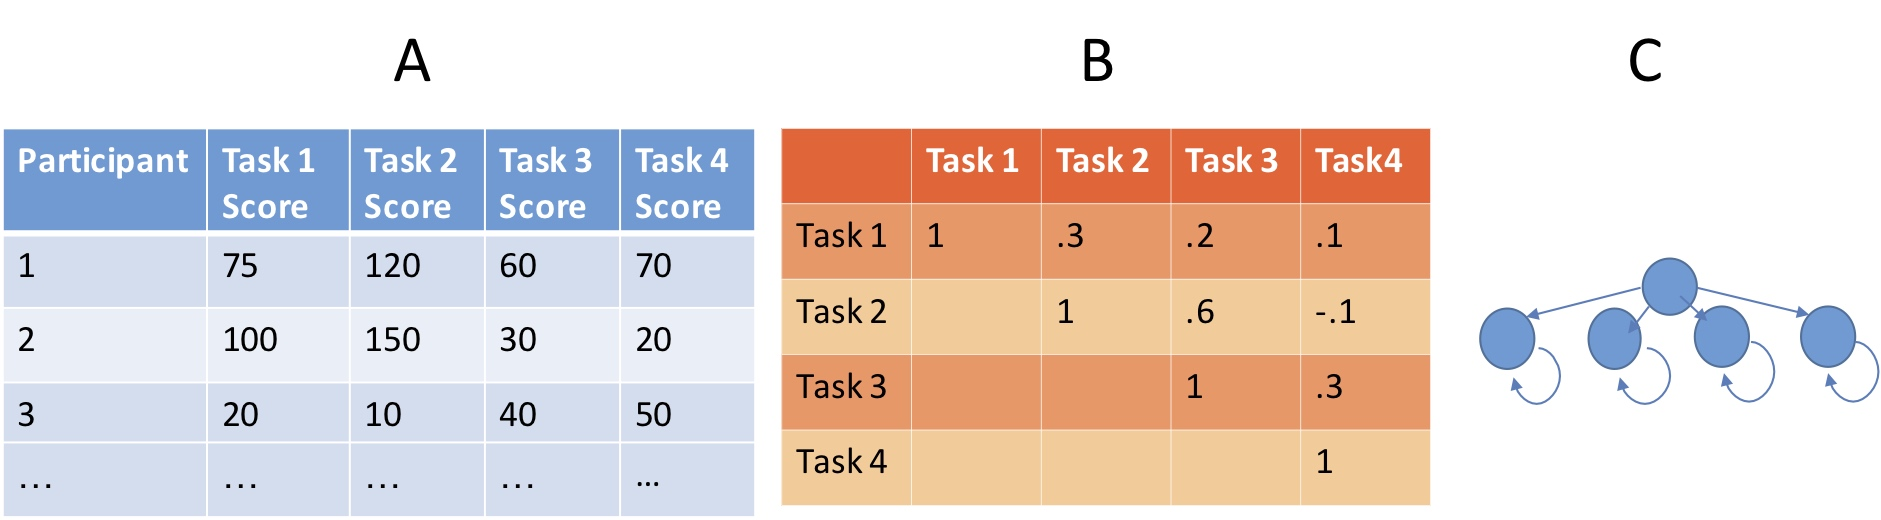
\includegraphics[width=5in]{dataAnalysis} \caption{Usual analysis: The raw data are used to tabulated into individual scores (A). The covariation among these individual scores may be computed (B).  These covariances are decomposed with structural equation models (C).}\label{fig:usual}
\end{figure}

Psychologists have long known that the ability to study covariation across tasks depends on the \emph{reliability} of each task (Spearman, 1904). If tasks have low reliability, then correlations are attenuated and it is difficult to extract the underlying latent structure of covariation. Indeed, most traditional task-based effects, say Stroop tasks or flanker tasks, are characterized by low reliability (Enkavi et al., 2019; Hedge, Powell, \& Sumner, 2018). We, along with others, worry that there is a \emph{reliability crisis} in the field of individual differences with traditional cognitive tasks. There are two signatures to this crisis: First, in the domain of cognitive control, several tasks that purportedly measure the same construct do not correlate well. For example, the correlation between flanker and Stroop effects in large studies is often near .1 and rarely greater than .25 (Enkavi et al., 2019; Rey-Mermet et al., 2018; Rouder, Haaf, \& Kumar, in preparation). These results indicate that even if these tasks are truly correlated, the correlation is not recoverable from low-task reliability. Second, extant latent-variable decompositions in cognitive-control domains seem unstable. This instability is showcased by Karr et al. (2018) who show that published latent-variable analyses with cognitive-control tasks are often unreplicable.

There are several recent proposed solutions to the reliability crisis including avoiding difference scores (Draheim, Mashburn, Martin, \& Engle, 2019), using diffusion models for combining speed and choice variables (Haines et al., 2020; Lerche et al., 2020), and making video-game versions of tasks (Deveau, Jaeggi, Zordan, Phung, \& Seitz, 2015; Kucina et al., 2022). An additional proposal---one that we have advocated---is to use hierarchical models to appropriately partition variability into distinct strata. The hope is that by modeling variability and covariability due to trials, conditions, tasks, and people, researchers can improve their recovery of correlations across tasks even in low-reliability environments (Haines et al., 2020; Matzke et al., 2017; Rouder \& Haaf, 2019). Indeed, there is good news on this front---hierarchical models outperform their nonhierarchical competitors and, perhaps more importantly, provide reasonable estimates of uncertainty (Rouder et al., in preparation). Even so, they provide no magic solution. It remains difficult to recover underlying latent structure in low-reliability environments.

Although we recommend hierarchical approaches in relatively simple cases (e.g., Rouder \& Haaf, 2019), they are not used in most applications. The reason is clear. It is not straightforward to incorporate both trial noise and structural-equation decompositions of covariance. There are no software packages that can conveniently combine trial noise and latent structures in the massively repeated designs that experimentalists use. To account for trial noise, it would be necessary to construct a separate node for each trial rather than start with person-by-task scores. While we think such hierarchical trial-noise + SEM decomposition models are tractable in principle, to our knowledge they have not been developed in the experimental-psychology context.

Our goal is not to promote tools that do not exist. Instead, we show here that the \emph{language} of hierarchical models, along with a few quick calculations, can provide a valuable tool in planning and interpreting individual-difference studies. In many ways, our goal is similar to Spearman (1904), who used the language of hierarchical models to develop his famous formula for disattenuating correlations. In some sense, our argument is an update on Spearman's with new features including variable trial sizes and a novel effect-size measure for reliability in the form of a signal-to-noise ratio.

To see the need for a new language, we need to look no further than the concept of \emph{reliability}. To show the problem, let's suppose two labs are studying the test-retest reliability of the Stroop effect with the same paradigm and materials. Each lab decides to run 200 people on Day 1 and then again on Day 2, perhaps a week later. Each lab computes each person's Stroop effect score by taking the difference between incongruent and congruent sample means, and each lab correlates these scores across Day 1 and Day 2 to estimate test-retest reliability. The only difference is that one lab decides to run 20 trials per person per day per condition; the other lab decides to run 200 trials per person per day per condition. It should be obvious that the procedure in the first lab yields a much lower test-retest reliability coefficient than the second lab because of the differences in the number of trials. Hence, the reliability coefficient is not a property of the task itself. It is not helpful to make statements such as ``The Stroop task has low reliability,'' because reliability is critically intertwined with the number of trials per person per condition (henceforth called \emph{trial size}).

This fact raises problems. Is the reliability crisis a crisis of trial size? What are appropriate trial sizes for localizing covariation across studies? Is there a measure of reliability that reflects the properties of the task without reference to trial size, and if so, what is it? What is the relationship between trial size, a trial-size invariant measure of reliability and the ability to localize correlations? Hierarchical models provide a clear insight into these questions, and that is why thinking about them both before and after analysis is important, even if they are not convenient or possible in a given context.

\hypertarget{reliability-as-signal-to-noise-ratios}{%
\section{Reliability as Signal-To-Noise Ratios}\label{reliability-as-signal-to-noise-ratios}}

To answer the above questions, we start with a simple hierarchical model of trial noise in a task.\footnote{Following convention, we distinguish between \emph{sample} and \emph{true} quantities. A sample quantity, say the sample mean, is observed and is affected by noise. A true quantity, say a true mean, exists in a large-sample limit and without noise. Sample quantities are statistics; true quantities are parameters. Following convention, we use Latin Letters for sample quantities, e.g., (\(\bar{Y}\)), and Greek letters for true quantities, e.g., \(\mu\).} Suppose \(I\) people each run \(L\) trials in congruent and incongruent conditions. Let \(i\) denote people, \(k\) denote conditions, and \(\ell\) denote replicate trials. Response times on trials serve as observations and are denoted \(Y_{ik\ell}\). Consider the model \(Y_{ik\ell} = \alpha_i +x_k\theta_i+\epsilon_{ik\ell}\), where \(x_k\) contrast codes condition and is -1/2 and 1/2 for congruent and incongruent conditions respectively. Parameter \(\alpha_i\) is the true overall speed of the \(i\)th participant. Parameter \(\theta_i\) is the true difference between incongruent and congruent conditions---it is the \(i\)th participant's true Stroop effect and the main target of analysis. The error term is \(\epsilon_{ik\ell} \sim \mbox{Normal}(0,\sigma^2)\), with \(\sigma^2\) describing the variability of trial noise. It is convenient to represent the model in random variable notion: \(Y_{ik\ell} \sim \mbox{Normal}(\alpha_i +x_k\theta_i,\sigma^2)\). The remaining critical specification is on \(\theta_i\), the true Stroop effect. Because each \(\theta_i\) describes a latent attribute of a person, it is reasonable to treat it as random effect: \(\theta_i \sim \mbox{Normal}(\nu,\delta^2)\) where \(\nu\) and \(\delta^2\) describe the population mean and variance. This last step makes the model hierarchical as variability across trials (\(\sigma^2\)) and across people (\(\delta^2\)) are modeled separately.

Most researcher do not start from
Researchers who perform the usual analysis (Fig. \ref{fig:usual}) compute sample means for each person for each condition, denoted \(\bar{Y}_{ik}\). Next, for each person, the congruent sample mean is subtracted from the incongruent sample mean to form a Stroop score, denoted \(d_i\), \(d_i=\bar{Y}_{i2}-\bar{Y}_{i1}\). It may seem that the sample mean and sample variance of these scores can be used to recover population means and variances. This, unfortunately, is not so, and stands at the root of poor performance with correlating individual differences in common cognitive-control tasks. According to the above model, the distribution of \(d_i\) is
\[d_i \sim \mbox{Normal}(\nu,\delta^2+2\sigma^2/L).\]\\
The mean of scores, \(\bar{d}\) estimates the population mean, but the variance of these scores does \emph{not} estimate \(\delta^2\), the population variance. Instead, there is an additional component from variability across trials, \(2\sigma^2/L\). It is this inflation of sample variance from trial noise that negatively influences reliability and correlation coefficients (Spearman, 1904). What follows is how this negative influence occurs and what may be done to mitigate it.

Consider a test-retest reliability paradigm and let \(j=1,2\) denote the day of data collection. Assuming everything remains constant except the trial noise, the test-retest model is \(Y_{ijk\ell} \sim \mbox{Normal}(\alpha_i +x_k\theta_i,\sigma^2)\). The distribution of Stroop effects for both days has common variability from \(\delta^2\) and unique variability from \(2\sigma^2/L\):

\begin{eq} \label{effectDist}
\begin{bmatrix}
d_{i1}\\ d_{i2}
\end{bmatrix}
\sim \mbox{N}_2\left(
\begin{bmatrix}\nu\\ \nu\end{bmatrix},
\begin{bmatrix} \delta^2+2\sigma^2/L & \delta^2\\ \delta^2 & \delta^2+ 2\sigma^2/L\end{bmatrix}\right),
\end{eq}

The test-retest reliability coefficient, \(r\), is the sample correlation coefficient between individuals' Stroop scores across days. From (\ref{effectDist}), the true correlation is \(\delta^2/(\delta^2+2\sigma^2/L)\). The sample test-retest coefficient \(r\), therefore, \emph{is estimating} \(\delta^2/(\delta^2+2\sigma^2/L)\), that is, the expected value or average of \(r\) across many such experiments is \(\E(r) \approx \delta^2/(\delta^2+2\sigma^2/L)\).\footnote{Sample correlations are not unbiased. For finite numbers of people, the exact equality does not hold, but with reasonable sized samples, the bias is reasonably small. In most individual-difference applications, researchers use relatively large numbers of people such that \(\E(r)\) well approximates its limit.} Sample reliability is a function of both trial-noise, between-participant variability, and trial size. As trial size increases, reliability to increases. The variability between-participants and within-trials determines the rate of increase.

What parts of reliability are invariant to trial size? Consider the ratio \(\delta^2/\sigma^2\). This is a signal-to-noise variance ratio---it is how much more variable people are relative to trial noise. Let \(\gamma^2\) denote this ratio.\\
With it, the reliability coefficient follows:
\[
\E(r)\approx\frac{\gamma^2}{\gamma^2+2/L}.
\]
The parameter \(\gamma^2\) serves as an effect-size measure of the reliability of the task.\footnote{The signal-to-noise variance ratio \(\gamma^2\), though an effect size, is quite different from more traditional effect size measures of \(\eta^2\) or \(\omega^2\). Effect size measure \(\eta^2\) and \(\omega^2\) are normalized by a total variance and are bounded above by 1.0. Measure \(\gamma^2\), on the other hand, is closer to \(F\) in meaning, but unlike \(F\), is not dependent on sample sizes. Measure \(\gamma^2\) is called \(g\) in Bayesian statistics (Zellner, 1986; Zellner \& Siow, 1980), and it plays a pivotal role of effect size in Bayesian analysis of linear and mixed-linear models (Liang, Paulo, Molina, Clyde, \& Berger, 2008; Rouder, Morey, Speckman, \& Province, 2012). We call this measure \(\gamma^2\) rather than \(g\) because it is a parameter and not an observable.} Tasks with high values of \(\gamma^2\) have variability across people that is greater than trial noise, and localizing individuals' effects may be done with just a small trial size. Tasks with low values of \(\gamma^2\) are difficult. It is hard to localize individuals' effects even with many trials, and recovering latent covariation across such tasks remains intractable in experiments with reasonable trial size. The parameter \(\gamma=\sqrt{\gamma^2}\) is the signal-to-noise standard-deviation ratio. It is often convenient for communication as standard deviations are sometimes more convenient than variance in communication.

Figure \ref{fig:rel} shows how signal-to-noise standard-deviation ratio \(\gamma\) and trial size affect the reliability coefficients. Large reliability coefficients can be achieved in a few trials for \(\gamma>1\); and somewhat high values can even be achieved in under \(L=100\) trials for \(\gamma>.25\). But tasks with lower signal-to-noise ratios may not be feasible as they require hundreds or thousands replicates per person per condition. The horizontal lines in Fig. \ref{fig:rel} may be used for planning. They show the trial sizes needed for reliability at criterial levels of .7 and .9. The problem then is to know what \(\gamma\) to use in planning experiments. We address this consideration subsequently.

\begin{figure}
\centering
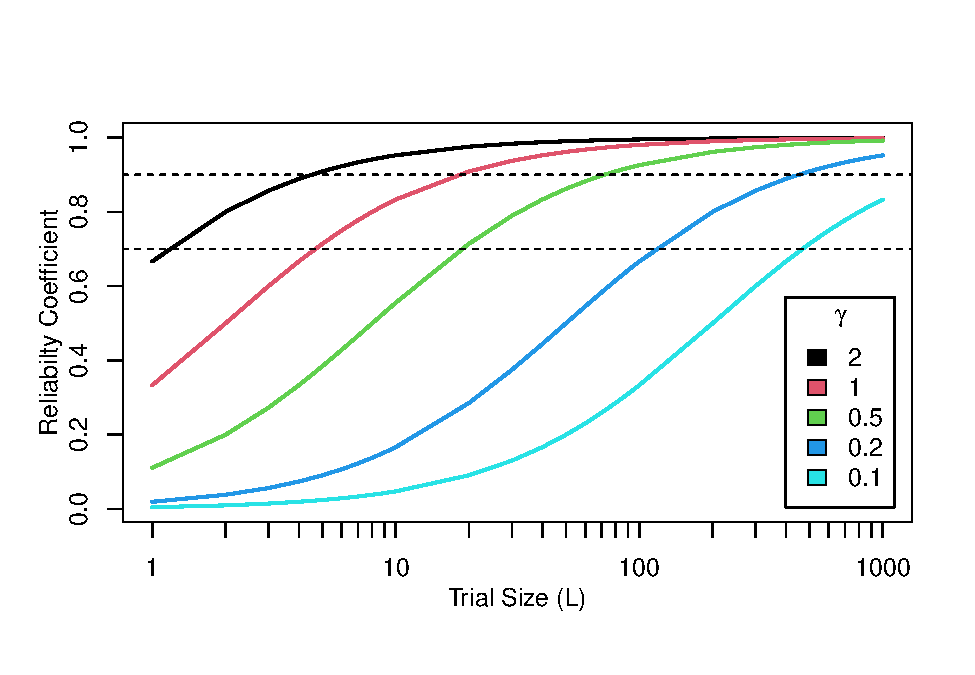
\includegraphics{p_files/figure-latex/rel-1.pdf}
\caption{\label{fig:rel}The expected value of reliability coefficients as a function of trial size for various signal-to-noise-standard-deviation ratios \(\gamma\). Horizontal lines at .7 and .9 can be used to plan the trial size for tasks with difference scores.}
\end{figure}

It is useful to see how trial size and signal-to-noise ratio affect correlation. Suppose we have two tasks, and let \(j\) indicate the task. Consider the model \(Y_{ijk\ell} \sim \mbox{Normal}(\alpha_{ij}+x_k\theta_{ij},\sigma^2_j)\), where there is true correlation, \(\rho\) across the tasks:
\[
\begin{bmatrix}
\theta_{i1}\\ \theta_{i2}
\end{bmatrix}
\sim \mbox{N}_2\left(
\begin{bmatrix}\nu_1\\ \nu_2\end{bmatrix},
\begin{bmatrix} \delta_1^2 & \rho\delta_1\delta_2\\\rho\delta_1\delta_2 & \delta_2^2\end{bmatrix}\right),
\]
The correlation between observed effects is
\[
\begin{bmatrix}
d_{i1}\\ d_{i2}
\end{bmatrix}
\sim \mbox{N}_2\left(
\begin{bmatrix}\nu_1\\ \nu_2\end{bmatrix},
\begin{bmatrix} \delta_1^2+2\sigma^2_1/L_1 & \rho\delta_1\delta_2\\\rho\delta_1\delta_2 & \delta_2^2+2\sigma^2_2/L_2\end{bmatrix}\right),
\]
where \(L_1\) and \(L_2\) are the trial sizes for the two tasks. The sample correlation, \(r\), estimates:
\[
\E(r) \approx \rho \left[\frac{\delta_1\delta_2}{\sqrt{(\delta_1^2+2\sigma^2_1/L_1)(\delta_2^2+2\sigma_2^2/L_2)}}\right] =
\rho \left[ \frac{\eta_1\eta_2}{\sqrt{(\eta_1^2+2/L_1)(\eta_2^2+2/L_2)}}\right].
\]
Hence, the sample correlation is attenuated, and the amount of attenuation depends both on the signal-to-noise variance ratio and the trial size. Often, if \(\gamma^2_1\) and \(\gamma^2_2\) are small, this attenuation is extreme even for reasonable trial sizes.

\hypertarget{the-consequences-of-low-and-high-signal-to-noise-in-practice}{%
\section{The Consequences of Low and High Signal-To-Noise In Practice}\label{the-consequences-of-low-and-high-signal-to-noise-in-practice}}

\begin{figure}
\centering
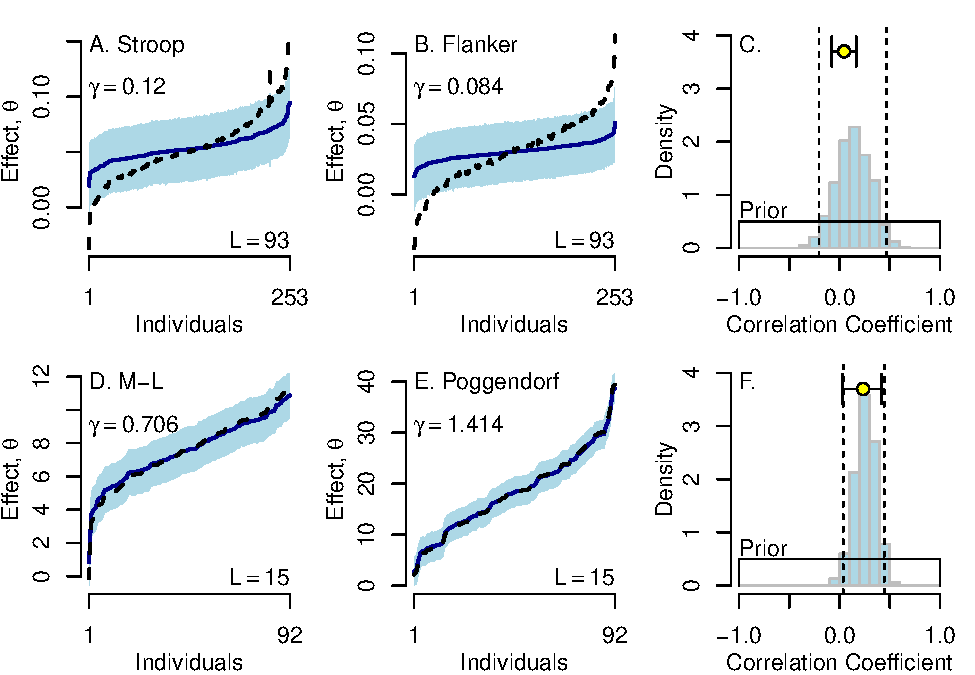
\includegraphics{p_files/figure-latex/reg-1.pdf}
\caption{\label{fig:reg}A-B. Observed effects (\(d_i\), dashed line) and model-based estimates (\(\theta_i\), solid line) for Rey Mermet et al.'s (2018) Stroop and flanker tasks. The shaded area shows the 95\% credible interval for model-based effects. The signal-to-noise ratio \(\gamma\) is low indicating much trial noise. C. Posterior distribution of model-based correlation (\(\rho\)) between Stroop and flanker effects. The dashed lines denote the 95\% credible interval. The point and segments above the distribution show the observed corrlelation coefficient and associated 95\% CI. D-E. Analogous plots for the Mueller-Lyar and Poggendorf illusions F. Anaologous plot for the correlation between Mueller-Lyar and Poggendorf effects.}
\end{figure}

To show the consequences of low and high signal-to-noise ratios, we analyze data from a cognitive-control battery and a visual-illusions battery. For each battery, we followed two analysis pathways. One is the usual pathway (Fig \ref{fig:usual}) in which the analysis starts from person-by-task sample effects, and observed correlations among these are the targets. The other pathway is model-based. Here we fit the simple hierarchical model that models trial noise along with participant noise. The hierarchical model may be analyzed by both frequentist (mixed-linear effect models, Pinheiro \& Bates, 2000) and Bayesian (Gelman, Carlin, Stern, \& Rubin, 2004) methods, and we chose the latter for convenience.

\hypertarget{cognitive-control}{%
\subsection{Cognitive control}\label{cognitive-control}}

The cognitive-control tasks come from Rey-Mermet et al. (2018), who had young and elderly participants perform a large battery. We highlight data from a number-Stroop task and a letter-flanker task. Fig. \ref{fig:reg}A shows the model analysis from the Stroop task. Plotted are observed effects \(d_i\) and model estimates of \(\theta_i\). Here, the two estimators differ, and the model estimators are far more compact or regularized than the corresponding sample effects.\\
Some readers will see regularization as a drawback as it compresses individual differences. This view is unwise. The large degree of regularization means that the apparent individual differences in sample effects are due to trial noise and are unreplicable. Fig. \ref{fig:reg}A shows the model estimate of \(\gamma\) (\(\hat{\gamma}=\)
0.12), and the number of trials (\(L=93\)). Even though there is a relatively large number of trials per person per condition and a large number of participants, the low signal-to-noise ratio implies that it is difficult to localize individual differences or recover any latent structure. Figure \ref{fig:reg}B shows the same for the flanker task; the signal-to-noise ratio is even lower than that for the Stroop task.

Figure \ref{fig:reg}C shows the correlation among tasks. The observed correlation and associated 95\% CI is shown as a large dot and horizontal line near the top of the distribution. The correlation value is known to be attenuated, and the relatively narrow CI reflects the large number of participants without consideration of trial noise. Unfortunately, this high degree of confidence is misplaced. The posterior distribution of \(\rho\) from the hierarchical model is plotted along with 95\% credible intervals. The uncertainty from low signal-to-noise ratios in the tasks is reflected in the large degree of uncertainty in correlation. Of note, the observed correlation, 0.045 is attenuated by a factor of 3.06 compared to the hierarchical estimate of 0.139. Moreover, the CI for the observed correlation is 37\% that of the credible interval from the hierarchical estimate showing much confidence in an attenuated value. In summary, low signal-to-noise ratios result in much uncertainty when trial noise is considered and much overconfidence in an attenuated value when trial noise is ignored. It is not a good situation.

\hypertarget{visual-illusions}{%
\subsection{Visual Illusions}\label{visual-illusions}}

The bottom row of Figure \ref{fig:reg} shows a much more sanguine case. The data are from a pilot study on visual illusions gathered by the authors and Michael S. Pratte. The paradigm for the illusions is shown in Figure \ref{fig:ill}. For the Muelller-Lyar paradigm, participants adjusted a center arrow so that it bisects the horizontal line. Participants' tendency here is to set the center arrow too far to the left, and we coded that as a positive bias. For the Poggendorf paradigm, participants adjusted the vertical offset of the right segment so that it lined up with the extension of the left segment through the occluded region. Participants' tendency is to set this segment too far down, and we coded this as a positive bias. A total of 100 individuals from Prolific ran 15 trials in each illusion; of these 100, 7 were discarded for producing uninterpretable data.\footnote{The illusion paradigm does not rely on a contrast between conditions. As a result, the reliability correlation is \(\E(r)\approx\gamma^2/(\gamma^2+1/L)\).}

The resulting biases in perception are shown in Figure\ref{fig:reg}D-E. As can be seen, illusion tasks yield quite high signal-to-noise ratios. These high-ratio agree well with Cretenoud, Grzeczkowski, Kunchulia, and Herzog (2021), who studied individual differences in Mueller-Lyar, Ebbinghaus, and Ponzo illusions. With high signal-to-noise ratios, there is little regularization and sample mean estimates match hierarchical estimates even with the limited number of trials. Moreover, with high signal-to-noise ratios, observed and model correlations match in both value and uncertainty (Fig. \ref{fig:reg}F). In this case, because trial noise is small relative to individual variation, the uncertainty in correlation reflects the moderate number of people rather than the limited number of trials.

\begin{figure}
\centering
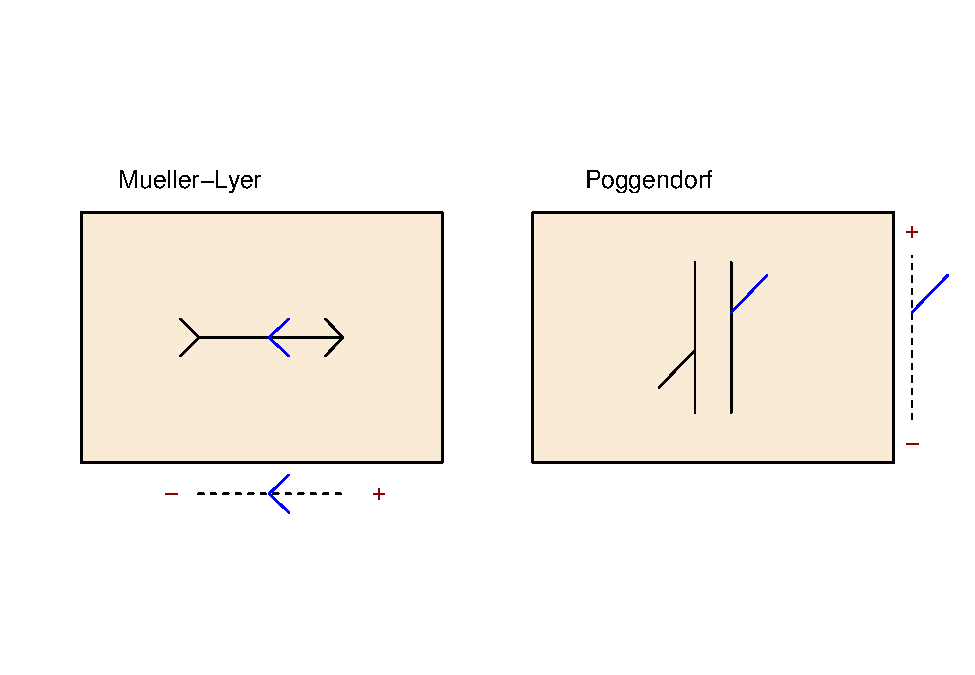
\includegraphics{p_files/figure-latex/ill-1.pdf}
\caption{\label{fig:ill}Paradigms for assessing visual illusions. Left: For the Muelller-Lyar paradigm, participants adjusted a center arrow so that it bisects the horizontal line. Right: For the Poggendorf illusion, participants adjusted the vertical offset of the right segment so that it lined up with the extension of the left segment through the occluded region.}
\end{figure}

\hypertarget{quick-calcuations-of-signal-to-noise-ratios}{%
\section{Quick Calcuations of Signal-To-Noise Ratios}\label{quick-calcuations-of-signal-to-noise-ratios}}

Although we estimated signal-to-noise ratios in the context of a Bayesian hierarchical model, it is possible to derive straightforward formula for these ratios without performing any model analysis. The case is similar to Spearman's derivation of the formula for disattenuating correlations. Spearman's formula is based on a similar hierarchical and one does not have to perform a hierarchical model analysis to use it.

Recall that for a single task, the sample effect, \(d_i\), is distributed as \(d_i\sim \mbox{Normal}(\nu,2\sigma^2/L+\delta^2)\). Hence, the usual sample variance has an expectation of
\(\mbox{E}[\mbox{Var}(d)]=2\sigma^2/L+\delta^2\). Substituting in \(\gamma^2\) yields, \(\mbox{E}[\mbox{Var}(d)]=\sigma^2(2/L+\gamma^2)\). Rearranging yields the following moments-based estimator of \(\gamma^2\):

\begin{eq} \label{sampGammaTask}
\hat{\gamma}^2 = \frac{\mbox{Var}(d)}{\hat{\sigma}^2}-\frac{2}{L},
\end{eq}

where \(\mbox{Var}(d)\) is the sample variance, \(\sum_i (d_i-\bar{d})^2/(I-1)\), and \(\hat{\sigma}^2\) is the MSE given by \(\sum_{ijk} (Y_{ijk}-\bar{Y}_{ij})^2/(IJ(K-1))\). For measures without contrasts, the analogous formula is

\begin{eq} \label{sampleGammaMeas}
\hat{\gamma}^2 = \frac{\mbox{Var}(d)}{\hat{\sigma}^2}-\frac{1}{L},
\end{eq}

We call estimates from (\ref{sampGammaTask}) and (\ref{sampleGammaMeas}) the sample estimates to distinguish them from model-based estimates.

Sample estimates of \(\gamma\) are, respectively, 0.12, and 0.07 for the Stroop and flanker tasks, and, respectively, 0.70, and 1.41, for the Mueller-Lyar and Poggendorf illusions. These values are very close to the model-based ones in Figure \ref{fig:reg}.

There is a potential issue with sample estimates. There is no guarantee that \(\hat{\gamma}^2\) is positive. The situation is analogous to that with Spearman's disattenuation formula. In Spearman's case, the disattenuated correlations were not guaranteed to be real numbers, and even when they were, they were not guaranteed to be in the {[}-1,1{]} interval. When these violations occurred, it indicated that the design was underpowered for the low-level of true reliability, and that the disattenuation was fraught with uncertainty. In our case, negative values of \(\hat{\gamma}^2\) too means that the design is underpowered for the low-level of true signal-to-noise ratio. The main advantages of Bayesian-model estimators in comparison are two-fold. First, resulting estimates are always in the valid range (between -1 and 1 for correlation; positive for \(\gamma^2\)). Second, estimates of correlation and signal-to-noise ratios come with uncertainties such as those in Figure \ref{fig:reg}.

\hypertarget{signal-to-noise-ratios-in-a-few-tasks-and-measures}{%
\section{Signal-To-Noise Ratios In A Few Tasks and Measures}\label{signal-to-noise-ratios-in-a-few-tasks-and-measures}}

The critical quantity for planning experiments and understanding the ability to localize correlations is \(\gamma\), the signal-to-noise ratios. What are the values for a range of tasks? Table\textasciitilde{} provides some guidance

\begin{table}[tbp]

\begin{center}
\begin{threeparttable}

\caption{\label{tab:allTasks}}

\begin{tabular}{lccccc}
\toprule
 & \multicolumn{1}{c}{Design} & \multicolumn{2}{c}{Signal-To-Noise SD
                        Estimates} & \multicolumn{2}{c}{Needed Trial Size} \\
\cmidrule(r){2-2} \cmidrule(r){3-4} \cmidrule(r){5-6}
Tasks & \multicolumn{1}{c}{Contrast} & \multicolumn{1}{c}{Sample} & \multicolumn{1}{c}{Model} & \multicolumn{1}{c}{r = 0.7} & \multicolumn{1}{c}{r = 0.9}\\
\midrule
Body Measure &  &  &  &  & \\
\ \ \ 1. Weight & N & 11.48 & - & 1 & 1\\
Stroop &  &  &  &  & \\
\ \ \ 2. Effect & Y & 0.18 & 0.12 & 158 & 607\\
\ \ \ 3. Speed & N & 0.96 & 0.96 & 3 & 10\\
Flanker &  &  &  &  & \\
\ \ \ 4. Effect & Y & 0.15 & 0.08 & 353 & 1359\\
\ \ \ 5. Speed & N & 0.70 & 0.7 & 5 & 19\\
Lexical Distance &  &  &  &  & \\
\ \ \ 6. Effect & Y & 0.16 & 0.11 & 193 & 742\\
\ \ \ 7. Speed & N & 0.60 & 0.62 & 7 & 24\\
Illusions &  &  &  &  & \\
\ \ \ 8. Mueller-Lyar & N & 0.72 & 0.71 & 5 & 19\\
\ \ \ 9. Poggendorf & N & 1.46 & 1.41 & 2 & 5\\
\bottomrule
\addlinespace
\end{tabular}

\begin{tablenotes}[para]
\normalsize{\textit{Note.} The standard deviation of repeated weight measurements was assumed at 3 lbs.}
\end{tablenotes}

\end{threeparttable}
\end{center}

\end{table}

The first row is for weight. We used the Army's 2011 survey of 6068 soldiers' weights. The mean and standard deviation are 175.40 lbs and 34.40 lbs, respectively. How variable are weight measurements? Modern human body scales may be accurate to half a pound or less, but some variation is expected for how the participant is balanced and recent food intake or exercise. Let's assume that a repeat measurement taken at some point in the same day might have a standard deviation of 3 lbs. This is a small amount relative to the variation across participants yielding an estimate of \(\gamma =\) 11.48. Weight is a best-case scenario, by far. The range of human weights compared to the accuracy of scales is indeed quite large.

The remainder of the rows come from the few tasks presented here plus one additional lexical distance task from Rouder, Lu, Speckman, Sun, and Jiang (2005). The next rows are for the Rey-Mermet et al.~Stroop task, and Row 2 shows the signal-to-noise ratio for the Stroop effect. As has been noted previously, the signal-to-noise ratio is low for the contrast between congruent and incongruent conditions. In the following row, Row 3, is for the average or overall speed.\footnote{The model is \(Y_{ik\ell} \sim \mbox{N}(\alpha_i+x_k\theta_i,\sigma^2)\) where both \(\alpha_i\) (speed) and \(\theta_i\) (effect) are treated as random effects: \(\alpha_i \sim \mbox{N}(\nu_\alpha,\gamma^2_\alpha\sigma^2)\) and \(\theta_i \sim \mbox{N}(\nu_\theta,\gamma^2_\theta\sigma^2)\). Posterior means of \(\gamma_\theta\) and \(\gamma_\alpha\) are shown in Table\textasciitilde{}\ref{tab:allTasks} for rows labeled \emph{Effect} and \emph{Speed}, respectively.} Here, the signal-to-noise ratio is great, that is, the variability in participants in overall speed is large relative to trial noise. Hence, only 10s of trials per person are needed to localize individual differences in speed.

There is one new task, lexical distance, which is an implementation of the distance-from-five effect (Moyer \& Landauer, 1967). Participants classified digits as either less-than or greater-than five, and did so more quickly if the digit was far from five (digits 2 and 8) than close to five (digits 4 and 6). The contrast row is for the contrast between near and far digits; the speed row is for the overall speed. As with cognitive-control tasks, the signal-to-noise is much greater for localizing individual overall speed effects than for localizing individual distance-from-five effects.

\hypertarget{the-reliability-crisis-revisited}{%
\section{The Reliability Crisis Revisited}\label{the-reliability-crisis-revisited}}

In this paper, we provide a novel reliability measure for experimental tasks. Unlike the common reliability coefficient, this measure is not dependent on trial size. The measure is a signal-to-noise variance ratio, denoted \(\gamma^2\). With it, researchers can communicate clearly about reliability without recourse to trial size. Signal-to-noise ratios succinctly indicate how well individual differences may be localized and how well the structure of covariation of individual differences across tasks may be recovered.

The motivation for the signal-to-noise ratio comes from a hierarchical treatment of variation across people, conditions, and trials. Even so, researchers need not analyze data with hierarchical models to use signal-to-noise ratios in planning experiments or interpreting results. We provide an easy-to-use estimator based on ordinary sample statistics. With it, signal-to-noise ratios may be used to characterize the reliability of tasks and to understand whether small correlation values reflect true structure or excessive trial noise. The advantage of hierarchical models is that they provide measures of uncertainty on correlations across tasks.

The cause of the reliability crisis is that researchers tend to use too few trials in tasks with too low signal-to-noise ratios. One obvious solution is to use more trials. For example, the correlation between Stroop and flanker can be well localized with \(L=500\) trials per person per condition. The problem with this obvious solution is that increasing trial size is often unrealistic or inconvenient. Some of the drawbacks to great numbers of trials are that fewer tasks may be run in a battery, conflict effects may attenuate with practice, and people may fatigue or even withdraw. Our motivation for avoiding excessive trial sizes is that we feel bad seeing our participants suffer through so much boredom.

There are other proposed solutions to the reliability crisis that are not as draconian as implementing excessive trial sizes. These include avoiding difference scores (Draheim et al., 2019), gamification (Deveau et al., 2015; Kucina et al., 2022), and diffusion modeling (Haines et al., 2020; Lerche et al., 2020; von Krause, Lerche, Schubert, \& Voss, 2020; Weigard, Clark, \& Sripada, 2021). Understanding the concept of task signal-to-noise helps in part to evaluate these proposals.

\hypertarget{avoiding-difference-scores}{%
\subsection{Avoiding Difference Scores}\label{avoiding-difference-scores}}

Draheim et al. (2019) recommends avoiding difference scores as raw input to latent variable analyses. Instead, they recommend using overall performance, for example, the average Stroop accuracy (in a difficult task) rather than the difference between conditions. We think there is much wisdom to this recommendation as signal-to-noise ratios are much higher for overall performance than for effects (see Table \ref{tab:allTasks}). Researchers who take this approach can use signal-to-noise ratios to plan their trial sizes. We suspect that the needed trial sizes will be delightfully small, and the ability to have quick and agile experiments may make the exploration of individual differences more tractable.

Nonetheless, this recommendation, while methodologically sound, comes with drawbacks. Difference scores are not at the root of the problem. In fact, our model reveals the same problems of low signal-to-noise for Stroop effects even though at no point were means subtracted. The issue is with experimental control. In a Stroop task, the contrast between congruent and incongruent is used to control nuisance factors such as overall processing speed, motivation, or conscientiousness. By focusing on the contrast, these nuisance factors are controlled, and the difference reflects only processes that systematically vary across conditions, such as the need for cognitive control. Performance measures that do not involve this contrast are assuredly confounded by nuisance factors. And individual differences in them may arise from individual differences in these nuisance factors rather than in cognitive control. We implore researchers who use overall performance scores or other measures without contrasts to be duly cautious in their interpretations about the theoretical source of individual differences.

\hypertarget{gamification}{%
\subsection{Gamification}\label{gamification}}

One innovation in cognitive control is the use of so-called \emph{gamified} tasks (Deveau et al., 2015; Kucina et al., 2022; Wells et al., 2021). When a task is gamified, it is made into a video game. There may be sound, color, theme music, point scores, leaderboards, and other elements of video-game play. There are two possible advantages of gamification. The first is that gamified tasks may be more reliable in that they have higher signal-to-noise ratios, \(\gamma^2\) (Kucina et al., 2022; Wells et al., 2021). For example, Wells et al. (2021) claim that the increased arousal and engagement from gamification results in more reliable data. Kucina et al. (2022) note that it may be possible to have combined stimulus elements in gamified settings that increase conflict effects. The second possible advantage is that people may be willing to engage with a gamified task at a higher level for longer (Deveau et al., 2015). Gamification then may be an effective tactic for increasing trial size without tears.

The development here provides an ideal language to assess whether gamification results in more reliable tasks. Any gain in reliability (as measured by a reliability coefficient) may be factored into that from increased trials and that from increased signal-to-noise ratios.

\hypertarget{diffusion-model-analysis}{%
\subsection{Diffusion-model analysis}\label{diffusion-model-analysis}}

The study of individual differences is inherently a psychometric or measurement endeavor. A relatively new approach is cognitive psychometrics (Batchelder, 2010) where plausible models of cognitive processes are used to improve the measurement of cognitive abilities. An advantage here is in interpretation---the target of inference is individual differences in theoretically meaningful cognitive processes as specified by explicit models. The most successful of these is Ratcliff's diffusion model of perception (Ratcliff, 1978). The latent parameter \emph{drift rate} captures the rate of information accumulation in a cognitive task. Diffusion models have been used to understand individual differences in aging (Ratcliff, Thapar, \& McKoon, 2001), psychopathology (White, Ratcliff, Vasey, \& McKoon, 2010), and cognitive control (Weigard et al., 2021). Moreover, Bayesian hierarchical models are convenient (Vandekerckhove, Tuerlinckx, \& Lee, 2011), and such, hierarchical regularzation in low-reliability tasks is possible. JEFF CITES.

One intriguing claim is that the individual differences in drift rate are more precisely located than individual differences in speed or accuracy alone (Lerche et al., 2020; Weigard et al., 2021). The claim is controversial as Enkavi et al. (2019) found only marginally higher reliability coefficients for drift rates vs.~RT alone. Even if the diffusion model parameters better locate individual differences, it is not clear that this potential improvement is sufficient for adequate localization in low-reliability tasks such as Stroop or flanker.

\hypertarget{concluding-thoughts}{%
\subsection{Concluding Thoughts}\label{concluding-thoughts}}

Where are there large individual differences in cognition? The question can more precisely be asked---what tasks or instruments have high signal-to-noise ratios, \(\gamma\)? Let's call these high-signal instruments, and examples of high-signal instruments include overall speed and biases in visual illusions. We advocate a prioritization of high-signal instruments even at the expense of more traditional instruments such as Stroop, flanker and Simon task effects. Even without these low-signal instruments, there is a rich cognitive worldthat can be explored fruitfully with individual differences. For example, what is the factor structure of overall speed across a wide range of tasks? Is there a general-susceptibility-to-illusions factor? We hope the development here provides the formal background for identifying high-signal instruments with cognitive tasks and speeds up this more fruitful exploration.

\newpage

\hypertarget{references}{%
\section*{References}\label{references}}
\addcontentsline{toc}{section}{References}

\hypertarget{refs}{}
\begin{CSLReferences}{1}{0}
\leavevmode\vadjust pre{\hypertarget{ref-Batchelder.2010}{}}%
Batchelder, W. H. (2010). Cognitive psychometrics: {Using} multinomial processing tree models as measurement tools. In S. E. Embretson (Ed.), \emph{Measuring psychological constructs: {Advances} in model-based approaches.} (pp. 71--93). {American Psychological Association}. Retrieved from \url{https://doi.org/10.1037/12074-004}

\leavevmode\vadjust pre{\hypertarget{ref-Bollen.1989}{}}%
Bollen, K. A. (1989). \emph{Structural equations with latent variables}. {Wiley}.

\leavevmode\vadjust pre{\hypertarget{ref-Cohen.etal.1994}{}}%
Cohen, J. D., Forman, S. D., Braver, T. S., Casey, B. J., Servan-Schreiber, D., \& Noll, D. C. (1994). Activation of the prefrontal cortex in a nonspatial working memory task with functional {MRI}. \emph{Human Brain Mapping}, \emph{1}(4), 293--304. doi:\href{https://doi.org/10.1002/hbm.460010407}{10.1002/hbm.460010407}

\leavevmode\vadjust pre{\hypertarget{ref-Cretenoud.etal.2021}{}}%
Cretenoud, A. F., Grzeczkowski, L., Kunchulia, M., \& Herzog, M. H. (2021). Individual differences in the perception of visual illusions are stable across eyes, time, and measurement methods. \emph{Journal of Vision}, \emph{21}(5), 26--26.

\leavevmode\vadjust pre{\hypertarget{ref-Deveau.etal.2015}{}}%
Deveau, J., Jaeggi, S. M., Zordan, V., Phung, C., \& Seitz, A. R. (2015). How to build better memory training games. \emph{Frontiers in Systems Neuroscience}, \emph{8}, 243.

\leavevmode\vadjust pre{\hypertarget{ref-Draheim.etal.2019}{}}%
Draheim, C., Mashburn, C. A., Martin, J. D., \& Engle, R. W. (2019). Reaction time in differential and developmental research: {A} review and commentary on the problems and alternatives. \emph{Psychological Bulletin}, \emph{145}(5), 508.

\leavevmode\vadjust pre{\hypertarget{ref-Engle.etal.1999}{}}%
Engle, R. W., Tuholski, S. W., Laughlin, J. E., \& Conway, A. R. A. (1999). Working {Memory}, {Short Term Memory}, and {General Fluid Intelligence}: {A} latent variable approach. \emph{Journal of Experimental Psychology: General}, \emph{128}, 309--331.

\leavevmode\vadjust pre{\hypertarget{ref-Enkavi.etal.2019}{}}%
Enkavi, A. Z., Eisenberg, I. W., Bissett, P. G., Mazza, G. L., MacKinnon, D. P., Marsch, L. A., \& Poldrack, R. A. (2019). Large-scale analysis of test--retest reliabilities of self-regulation measures. \emph{Proceedings of the National Academy of Sciences}, \emph{116}(12), 5472--5477.

\leavevmode\vadjust pre{\hypertarget{ref-Eriksen.Eriksen.1974}{}}%
Eriksen, B. A., \& Eriksen, C. W. (1974). Effects of noise letters upon the identification of a target letter in a nonsearch task. \emph{Perception \& Psychophysics}, \emph{16}, 143--149.

\leavevmode\vadjust pre{\hypertarget{ref-Gelman.etal.2004}{}}%
Gelman, A., Carlin, J. B., Stern, H. S., \& Rubin, D. B. (2004). \emph{Bayesian data analysis (2nd edition)}. {London}: {Chapman and Hall}.

\leavevmode\vadjust pre{\hypertarget{ref-Haines.etal.2020}{}}%
Haines, N., Kvam, P. D., Irving, L. H., Smith, C., Beauchaine, T. P., Pitt, M. A., \ldots{} Turner, B. M. (2020). Theoretically informed generative models can advance the psychological and brain sciences: {Lessons} from the reliability paradox.

\leavevmode\vadjust pre{\hypertarget{ref-Hedge.etal.2018}{}}%
Hedge, C., Powell, G., \& Sumner, P. (2018). The reliability paradox: {Why} robust cognitive tasks do not produce reliable individual differences. \emph{Behavioral Research Methods}.

\leavevmode\vadjust pre{\hypertarget{ref-Kane.etal.2001}{}}%
Kane, M. J., Bleckley, M. K., Conway, A. R. A., \& Engle, R. W. (2001). A controlled-attention view of working-memory capacity. \emph{Journal of Experimental Psychology: General}, \emph{130}(2), 169--183. Retrieved from \url{http://search.ebscohost.com/login.aspx?direct=true\&db=psyh\&AN=2001-17501-002\&loginpage=Login.asp\&site=ehost-live\&scope=site}

\leavevmode\vadjust pre{\hypertarget{ref-Karr.etal.2018}{}}%
Karr, J. E., Areshenkoff, C. N., Rast, P., Hofer, S. M., Iverson, G. L., \& Garcia-Barrera, M. A. (2018). The unity and diversity of executive functions: {A} systematic review and re-analysis of latent variable studies. \emph{Psychological Bulletin}, \emph{144}(11), 1147.

\leavevmode\vadjust pre{\hypertarget{ref-Kucina.etal.2022}{}}%
Kucina, T., Wells, L., Lewis, I., de Salas, K., Kohl, A., Palmer, M., \ldots{} Heathcote, A. (2022). A solution to the reliability paradox for decision-conflict tasks.

\leavevmode\vadjust pre{\hypertarget{ref-Lerche.etal.2020}{}}%
Lerche, V., von Krause, M., Voss, A., Frischkorn, G. T., Schubert, A.-L., \& Hagemann, D. (2020). Diffusion modeling and intelligence: {Drift} rates show both domain-general and domain-specific relations with intelligence. \emph{Journal of Experimental Psychology: General}, \emph{149}, 2207--2249. doi:\href{https://doi.org/10.1037/xge0000774}{10.1037/xge0000774}

\leavevmode\vadjust pre{\hypertarget{ref-Liang.etal.2008}{}}%
Liang, F., Paulo, R., Molina, G., Clyde, M. A., \& Berger, J. O. (2008). Mixtures of g-priors for {Bayesian Variable Selection}. \emph{Journal of the American Statistical Association}, \emph{103}, 410--423. Retrieved from \url{http://pubs.amstat.org/doi/pdf/10.1198/016214507000001337}

\leavevmode\vadjust pre{\hypertarget{ref-Matzke.etal.2017}{}}%
Matzke, D., Ly, A., Selker, R., Weeda, W. D., Scheibehenne, B., Lee, M. D., \& Wagenmakers, E.-J. (2017). Bayesian inference for correlations in the presence of measurement error and estimation uncertainty. \emph{Collabra: Psychology}, \emph{3}(1).

\leavevmode\vadjust pre{\hypertarget{ref-Miyake.etal.2000}{}}%
Miyake, A., Friedman, N. P., Emerson, M. J., Witzki, A. H., Howerter, A., \& Wager, T. D. (2000). The unity and diversity of executive functions and their contributions to complex {``frontal lobe''} tasks: {A} latent variable analysis. \emph{Cognitive Psychology}, \emph{41}(1), 49--100.

\leavevmode\vadjust pre{\hypertarget{ref-Moyer.Landauer.1967}{}}%
Moyer, R. S., \& Landauer, T. K. (1967). Time required for judgements of numerical inequality. \emph{Nature}, \emph{215}, 1519--1520.

\leavevmode\vadjust pre{\hypertarget{ref-Pinheiro.Bates.2000}{}}%
Pinheiro, J. C., \& Bates, D. M. (2000). \emph{Mixed-effects models in {S} and {S-PLUS}}. {New York}: {Springer}.

\leavevmode\vadjust pre{\hypertarget{ref-Ratcliff.1978}{}}%
Ratcliff, R. (1978). A theory of memory retrieval. \emph{Psychological Review}, \emph{85}, 59--108.

\leavevmode\vadjust pre{\hypertarget{ref-Ratcliff.etal.2001}{}}%
Ratcliff, R., Thapar, A., \& McKoon, G. (2001). The effects of aging on reaction time in a signal detection task. \emph{Psychology and Aging}, \emph{16}, 323--341.

\leavevmode\vadjust pre{\hypertarget{ref-Rey-Mermet.etal.2018}{}}%
Rey-Mermet, A., Gade, M., \& Oberauer, K. (2018). Should {We Stop Thinking About Inhibition}? {Searching} for {Individual} and {Age Differences} in {Inhibition Ability}. \emph{Journal of Experimental Psychology: Learning, Memory, and Cognition}. Retrieved from \url{http://dx.doi.org/10.1037/xlm0000450}

\leavevmode\vadjust pre{\hypertarget{ref-Rouder.Haaf.2019}{}}%
Rouder, J. N., \& Haaf, J. M. (2019). A psychometrics of individual differences in experimental tasks. \emph{Psychonomic Bulletin and Review}, \emph{26}(2), 452--467. Retrieved from \url{https://doi.org/10.3758/s13423-018-1558-y}

\leavevmode\vadjust pre{\hypertarget{ref-Rouder.etal.inpreparation}{}}%
Rouder, J. N., Haaf, J. M., \& Kumar, A. (in preparationin preparation). \emph{Why {Most Studies} of {Individual Differences With Cognitive Tasks Are Bound To Fail}}.

\leavevmode\vadjust pre{\hypertarget{ref-Rouder.etal.2005}{}}%
Rouder, J. N., Lu, J., Speckman, P. L., Sun, D., \& Jiang, Y. (2005). A {Hierarchical Model} for {Estimating Response Time Distributions}. \emph{Psychonomic Bulletin and Review}, \emph{12}, 195--223.

\leavevmode\vadjust pre{\hypertarget{ref-Rouder.etal.2012}{}}%
Rouder, J. N., Morey, R. D., Speckman, P. L., \& Province, J. M. (2012). Default {Bayes Factors} for {ANOVA Designs}. \emph{Journal of Mathematical Psychology}, \emph{56}, 356--374. Retrieved from \url{http://dx.doi.org/10.1016/j.jmp.2012.08.001}

\leavevmode\vadjust pre{\hypertarget{ref-Skrondal.Rabe-Hesketh.2004}{}}%
Skrondal, A., \& Rabe-Hesketh, S. (2004). \emph{Generalized {Latent Variable Modeling}: Multilevel, longitudinal, and structural equation models}. {Boca Raton}: {CRC Press}.

\leavevmode\vadjust pre{\hypertarget{ref-Spearman.1904a}{}}%
Spearman, C. (1904). The {Proof} and {Measurement} of {Association} between {Two Things}. \emph{American Journal of Psychology}, \emph{15}, 72--101. Retrieved from \url{https://www.jstor.org/stable/pdf/1412159.pdf}

\leavevmode\vadjust pre{\hypertarget{ref-Stroop.1935}{}}%
Stroop, J. R. (1935). Studies of interference in serial verbal reactions. \emph{Journal of Experimental Psychology}, \emph{18}, 643--662.

\leavevmode\vadjust pre{\hypertarget{ref-Vandekerckhove.etal.2011}{}}%
Vandekerckhove, J., Tuerlinckx, F., \& Lee, M. D. (2011). Hierarchical diffusion models for two-choice response time. \emph{Psychological Methods}, \emph{16}, 44--62.

\leavevmode\vadjust pre{\hypertarget{ref-vonKrause.etal.2020}{}}%
von Krause, M., Lerche, V., Schubert, A.-L., \& Voss, A. (2020). Do {Non-Decision Times Mediate} the {Association} between {Age} and {Intelligence} across {Different Content} and {Process Domains}? \emph{Journal of Intelligence}, \emph{8}(3, 3), 33. doi:\href{https://doi.org/10.3390/jintelligence8030033}{10.3390/jintelligence8030033}

\leavevmode\vadjust pre{\hypertarget{ref-Weigard.etal.2021}{}}%
Weigard, A., Clark, D. A., \& Sripada, C. (2021). Cognitive efficiency beats top-down control as a reliable individual difference dimension relevant to self-control. \emph{Cognition}, \emph{215}, 104818. doi:\href{https://doi.org/10.1016/j.cognition.2021.104818}{10.1016/j.cognition.2021.104818}

\leavevmode\vadjust pre{\hypertarget{ref-Wells.etal.2021}{}}%
Wells, L., Kucina, T., Kohl, A., Lewis, I., de Salas, K., Aidman, E., \& Heathcote, A. (2021). A flexible gaming environment for reliably measuring cognitive control. In \emph{Proceedings of the 2021 {Human Factors} and {Medicine Research Symposium-Applying Neuroscience} to {Performance}: {From Rehabilitation} to {Human Cognitive Augmentation}} (pp. 11--12).

\leavevmode\vadjust pre{\hypertarget{ref-White.etal.2010}{}}%
White, C. N., Ratcliff, R., Vasey, M. W., \& McKoon, G. (2010). Using diffusion models to understand clinical disorders. \emph{Journal of Mathematical Psychology}, \emph{54}(1), 39--52.

\leavevmode\vadjust pre{\hypertarget{ref-Zellner.1986}{}}%
Zellner, A. (1986). On assessing prior distirbutions and {Bayesian} regression analysis with g-prior distribution. In P. K. Goel \& A. Zellner (Eds.), \emph{Bayesian inference and decision techniques: {Essays} in honour of {Bruno} de {Finetti}} (pp. 233--243). {Amsterdam}: {North Holland}.

\leavevmode\vadjust pre{\hypertarget{ref-Zellner.Siow.1980}{}}%
Zellner, A., \& Siow, A. (1980). Posterior {Odds Ratios} for {Selected Regression Hypotheses}. In J. M. Bernardo, M. H. DeGroot, D. V. Lindley, \& A. F. M. Smith (Eds.), \emph{Bayesian {Statistics}: {Proceedings} of the {First International Meeting} held in {Valencia} ({Spain})} (pp. 585--603). {University of Valencia}.

\end{CSLReferences}


\end{document}
